\documentclass[11pt,english,a4paper]{scrartcl}

%\usepackage[utf8]{inputenc}   % Font Encoding, benoetigt fuer Umlaute
\usepackage[english]{babel}    % Spracheinstellung

%\usepackage[T1]{fontenc}     % T1 Schrift Encoding
\usepackage{textcomp}         % Zusatzliche Symbole (Text Companion font extension)
%\usepackage{lmodern}         % Latin Modern Schrift

\usepackage{amsmath,amssymb}  % mehr Mathe!
\usepackage{psfrag}           % Text in eps-Bildern ersetzen
\usepackage{url}              % Hyperlinks für urls
\usepackage{graphicx}
\usepackage{tabularx}
\usepackage{float}            % gleitende Objekte mit [H] wirklich HIER positionieren^
\usepackage{color}            % bring Farbe ins Leben =)
\usepackage{geometry}         % einfache Seiteneinrichtung
%\usepackage{subfigure}
%\usepackage{booktabs}
%\usepackage{framed}
\usepackage{fancyhdr}         % schicke Kopf- und Fußzeilen basteln
\usepackage{fancybox}	      % für runde Umrandungs-Boxen und solchen Crap
\usepackage{ifthen}	      % logische Abfragen
\usepackage{hyperref}         % interaktive hyperlinks für Querverweise
\usepackage{currfile}	      % get the current file name


%%%%%%% Flags for solutions: %%%%%%%%%%%%%%%%%%%%%%%%%%%%%%%%%%%%%%%%%%%
%\newboolean{Solution}
%\newboolean{longSol}



%%%%%% Seiteneinrichtung und Kopf/Fußzeilendefinition %%%%%%%%%%%%%%%%%%%
\geometry{a4paper,left=25mm,right=20mm,top=30mm,bottom=50mm}
% set indentation for paragraphs to zero:
\setlength{\parindent}{0pt}
% alle Kopf- und Fußzeilenfelder löschen:
\fancyhf{}
\setlength{\headwidth}{\textwidth}
\setlength{\headheight}{75pt}
% Linie in Kopfzeile ausblenden:
\renewcommand{\headrulewidth}{0.0pt}
\fancyfoot[R]{\sffamily \thepage}
% left footer only when detailed solutions are switched on:
%\ifthenelse{\boolean{longSol}}{
%  \fancyfoot[L]{\sffamily Aufgabe \theproblem}}{}
%% Linie Fußzeile:
%\renewcommand{\footrulewidth}{0.5pt}
%\renewcommand*\chapterheadstartvskip{\vspace{-\topskip}}
% Abstand zwischen Kapitelüberschrift und Seitenkopf verkleinern:
%\renewcommand*\chapterheadstartvskip{\vspace{-8ex}}

% Standardseitenstil (alle Seiten ohne Kapitelüberschrift) definieren:
%\fancyhead[L]{\iomHeader}

% plain-Seitenstil (für Seiten mit Kapitelüberschrift) überschreiben, so dass auch die erste Kapitelseite Kopf-und Fußzeile nach Maß bekommt:
%\fancypagestyle{plain}{\fancyhead[L]{\iomHeader}}

% Kopfzeile für IOM:
%\newcommand{\iomHeader}{
%  \sffamily
%  \begin{tabularx}{\textwidth}{lXr}
%  \hline
%  \,\includegraphics[height= 0.27cm]{imlogo} 
%  TU Dortmund -- Institut für Mechanik & & Prof. Dr.-Ing. Andreas Menzel\\   Mechanik für Maschinenbau & & Dipl.-Ing. Raphael Holtermann\\
%  \hline\\
%  \end{tabularx}
%}
%%%%%%%%%%%%%%%%%%%%%%%%%%%%%%%%%%%%%%%%%%%%%%%%%%%%%%%%%%%%%%%%%%%%%%%%%%

% diverses Zeug
\definecolor{greend}{rgb}{0.00,0.60,0.00} % dark grey
\definecolor{blued}{rgb}{0.00,0.00,0.60} % dark blue

\renewcommand{\vec}[1]{\ensuremath{\mbox{\boldmath $#1$}}}
\renewcommand{\d}{\operatorname{d}\negthinspace}
\newcommand{\smallsep}{\setlength{\itemsep}{-0.1\parsep}}
\newcommand{\bs}{\boldsymbol}

\newcommand{\eigenname}[1]{\textsc{#1}}
\newcommand{\begriff}[1]{\textbf{#1}}
\newcommand{\buchtitel}[1]{"\textit{#1}"}
\newcommand{\vit}{\eigenname{Vellore Institute of Technology}}



%%%%% Befehlsumgebungen für Aufgaben: %%%%%%%%%%%%%%%%%%%%%%%%%%%%%%%%%%%%%
%
%% Zähler für Aufgaben:
%\newcounter{problem}
%% der bei jedem neuen Kapitel  0 gesetzt wird:
%\numberwithin{problem}{chapter}
%
%% Befehl für Aufgaben:
%\newcommand{\problem}[4][width=0.8 \textwidth]{
% \addtocounter{problem}{1}
% 
% %insert page break if longsolution is provided
% \ifthenelse{\boolean{longSol}}{\newpage}{}
% \section*{Aufgabe \theproblem \ifthenelse{\boolean{longSol}}{\ [.../\currfiledir]}{}}
%  \noindent
%  \begin{minipage}{\textwidth}
%    \begin{minipage}[t]{0.5\textwidth}
%      #2
%    \end{minipage}
%    \hfill
%    %\mbox{\numexpr{0.95-#5}} geht vielleicht auch irgendwie
%    \begin{minipage}[t]{0.5\textwidth}				%ehemals 0.45 [LARS]
%      ~\\[-1ex]%fakezeile, um beide minipages mit der t-Zeile auszurichten
%      #4 %argumentliste mit psfrag-befehlen
%      \centerline{\includegraphics[#1]{#3}}
%    \end{minipage}
%  \end{minipage}
%}
%
%
%% umgebung für Aufgaben mit zweispaltigem Bild
%\newcommand{\bigproblem}[4][width=0.8 \textwidth]{
% \addtocounter{problem}{1}
% 
% %insert page break if longsolution is provided
% \ifthenelse{\boolean{longSol}}{\newpage}{}
% \section*{Aufgabe \theproblem}
% \begin{minipage}{\textwidth}
%  \noindent
%      #2 \bigskip
%      
%  {
%      #4 %argumentliste mit psfrag-befehlen
%      \centerline{\includegraphics[#1]{#3}}
%  }
%  \end{minipage}
%}
%
%\newcommand{\solution}[2]
%{
%  \ifthenelse{\boolean{Solution}}
%  {
%  \ifthenelse{\NOT\boolean{longSol}}
%    {%short solution
%     \vspace*{-2ex}
%     \paragraph{Lösung:} #1
%    }
%    {%long solution
%     \subsection*{Lösung:} #2
%    }
%  }
%  {%else; not used here
%  }
%}
%


\title{Cooperative Manipulators}
\author{Tobias Keute}

\begin{document}
\vfill
\maketitle
\thispagestyle{empty}
\vfill
\pagebreak
\tableofcontents
\thispagestyle{empty}
\pagebreak
\setcounter{page}{1}
\section{Introduction}
	\subsection{What is a Robot? What is a Manipulator?}
	At first sight a \begriff{robot} is very similar to a crane for example. Both are made from several \begriff{links} attached serialy with either revolute or prismatic \begriff{joints}, at both the end effector can be placed in any place in the \begriff{workspace} by defining the \begriff{joint parameters} of each individual joint. The only difference between a robot and a \begriff{manipulator} (the crane) is that the manipulator ist controlled by a human and the robot is guided by an program running on a computer.
%	\include{ArmAlsRoboter.ps}
%
%	
%	
%	\subsection{What is so important about robots being cooperative?}
%\section{Rigid Manipulators}
%\section{Cooperativ Rigid Manipulators}
\section{Flexible Manipulators}
	As the focus of modern manufactoring is more and more on light-weight tecnology, as for example 	
space schiences, the structures will lose their rigid character and become more and more flexible. For this reason it is necessary not only to calculate the rigid-body movements, but also simulate the deformations and use the results in the simulation of the movement of the robot. One, probably the most common, method of calculating this deformations I will show in the next subsection.
	\subsection{A short trip to Finite Elements Analysis (FEA)}
To calculate deformations and stresses of structures, \begriff{finite element analysis} is an important and often used method. It divides the structure in several points, calles \begriff{nodes}, and \begriff{elements} between those nodes. 
\bigskip

As the finite element analysis divides a part in very many elements and there are a lot of equations to solve for every node, the finite element analysis was not very popular until the 1950s. With the rise of the computer it was possible to solve thousands of equations in a few minutes. The more the computer was developed, the more programs for finite element analysis were developed.
\bigskip

In the following subsection I will give a short review about finite element analysis showing on the example of an one dimensional bar leading to methods of solving more complex problems of two- and three-dimensional problems.
\bigskip

Let us assume that the rod is on simple support and under a constant axial load of $q_0$, length $L$, Young's Module $E$ and cross-section area $A$:
\bigskip

\begin{center}
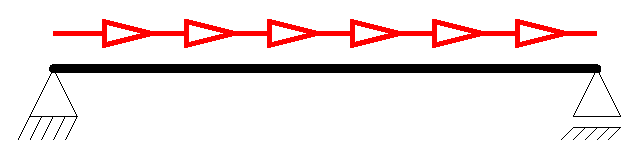
\includegraphics[scale=1]{OneDimensionalBar}
\end{center}
\bigskip
From the elementary courses of mechanics we know that
\begin{align}
EA\,\frac{du}{dx}+q_0=0 \label{Rod_Main}
\end{align}
As we now proceed we can assume any trial function $û(x)$ that satisfies the boundary conditions that $û=0$ at $x=0$ and $\frac{dû}{dx}=0$ at $x=L$.

Let $û$ be a polynomial function of $x$ with 
\begin{align}
û(x)=c_0\,+\,c_1\,x\,+\,c_2\,x \nonumber
\end{align}
with the unknown constants $c_0$, $c_1$ and $c_2$. According to the boundary conditions we have $c_0=0$ and $c_1=-c_2\,L$. Now our trial function looks like
\begin{align}
û(x)=-2c_2Lx\,+\,c_2x=c_2(x\,-\,2Lx) \nonumber
\end{align}
As we substitute $û$ in eq.\ref{Rod_Main} we come to the following equation:
\begin{align}
2AEc_2+q_0=R_d \nonumber
\end{align}
with $R_d$ as the \begriff{residual}. We see that for $c_2=\frac{-q_0}{2AE}$ the residual is equal to zero on every point of the rod. We will see later, that this will not happen for every trial function. As the residual is equal to zero on every point our solution is equal to the exact solution:
\begin{align}
û(x)=(2xL-x²)\frac{q_0}{2AE}=u(x) \nonumber
\end{align}
Assuming a different trial solution, e.g. $û(x)=c_0\,sin(\frac{\pi\,x}{2L})$, we see that the boundary conditions $û=0$ at $x=0$ and $\frac{dû}{dx}=0$ at $x=L$ are satisfied. As the equation has only one free parameter, $c_0$, it is called a \begriff{one-parameter solution}.

As we substitute $\frac{d^2û}{dx^2}$ again in eq.\ref{Rod_Main} we come to:
\begin{align}
-EA\, c_0\,sin\left(\frac{\pi\,x}{2L}\right)\frac{\pi^2}{4L^2}+q_0=R_d \nonumber
\end{align}

We see that there is no constant $c_0$ that makes $R_d$ equal to zero on every point of the rod. We can try to make $R_d$ equal to zero on one point (for example $x=0.5L$), but the errors would be quite huge. 

An opportunity to make the mistakes smaller is to add more parameters to our trial solution like
\begin{align}
û(x)=c_0\,sin\left(\frac{\pi\,x}{2L}\right)\,+\,c_1\,sin\left(\frac{3\,\pi\,x}{2l}\right)\,+\,c_2\,sin\left(\frac{5\,\pi\,x}{2L}\right)\,+... 
\end{align}
which decreases the mistake the more parameters we invent how fig.\ref{ExactVSParameter} shows. This technique is called the \begriff{point collocation technique}.

\bigskip
An other method is the \begriff{weighted residual technique}, where $W(x)$ is the \begriff{weighted function}. We will multiplicate the residual of our trial function with this weighted function and integrate it over the whole area. 
\begin{align}
\int\,W(x)\,R_d(x)\,dx=0 \nonumber
\end{align}
Theoretically we can chose every function as weighted function as long as they are integrable, but \eigenname{Galerkin} introduced the idea of letting $W(x)$ be $û(x)$ itself in 1915, which works pretty well with most problems (see fig.\ref{ExactVSGalerkin})

\bigskip
So for our problem with the one dimensional rod $W(x)$ will be
\begin{align}
W(x)=sin\left(\frac{\pi\,x}{2L}\right) \nonumber
\end{align}

And the integral would be
\begin{align}
\int\,sin\left(\frac{\pi\,x}{2L}\right)\,\left(-EA\, c_0\,sin\left(\frac{\pi\,x}{2L}\right)\frac{\pi^2}{4L^2}+q_0\right)\,dx=0 \nonumber
\end{align}
which will lead to
\begin{align}
c_0=\frac{16\,L^2q_0}{\pi^3EA} \nonumber
\end{align}
\bigskip

\begin{figure}[!h]
\begin{center}
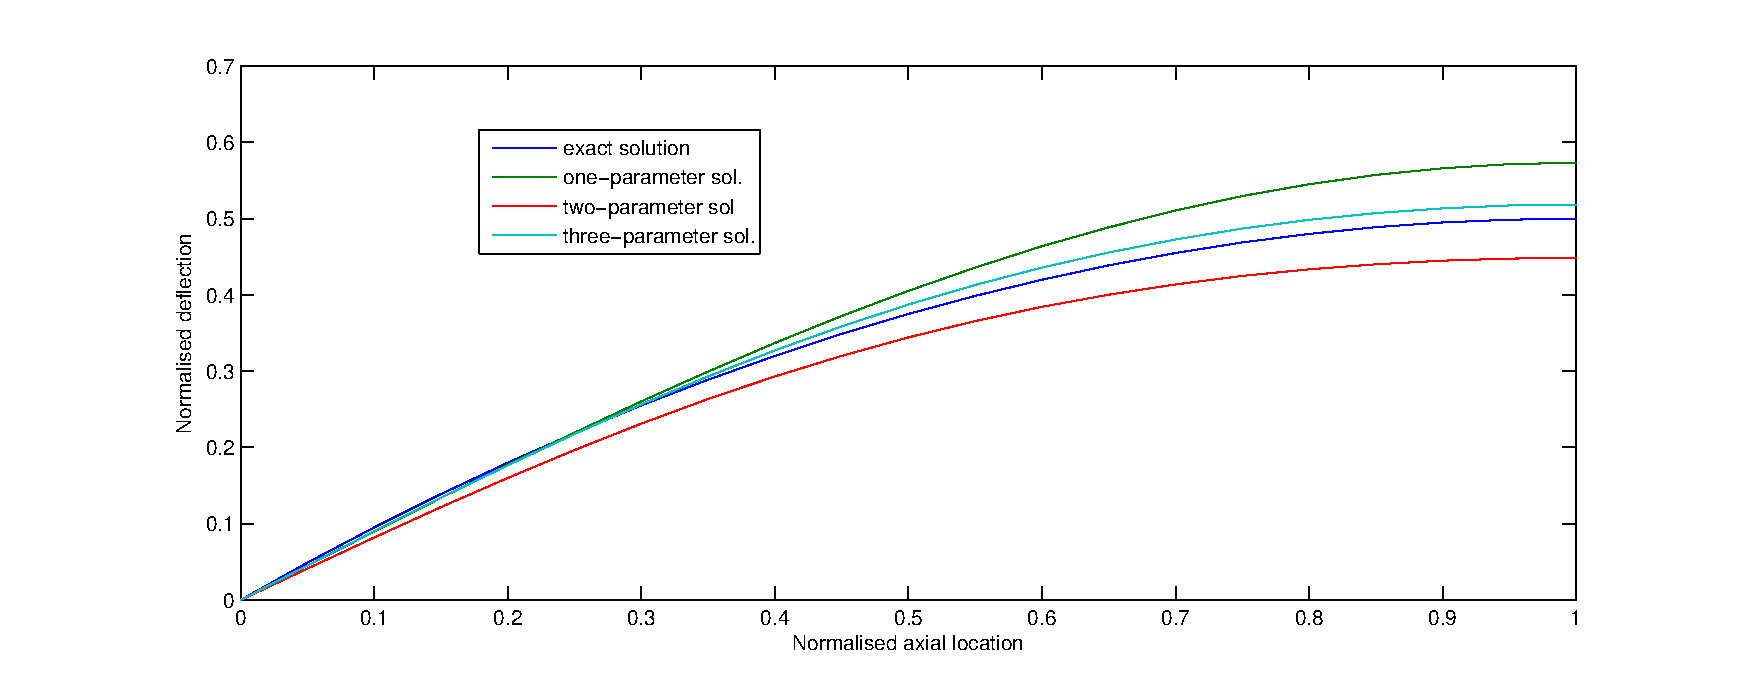
\includegraphics[scale=0.5]{ExactVSParameter} 
\caption{The exact solution compared to the one-, two-, and three-parameter solution}
\label{ExactVSParameter}
\end{center}
\end{figure}
\begin{figure}[!h]
\begin{center}
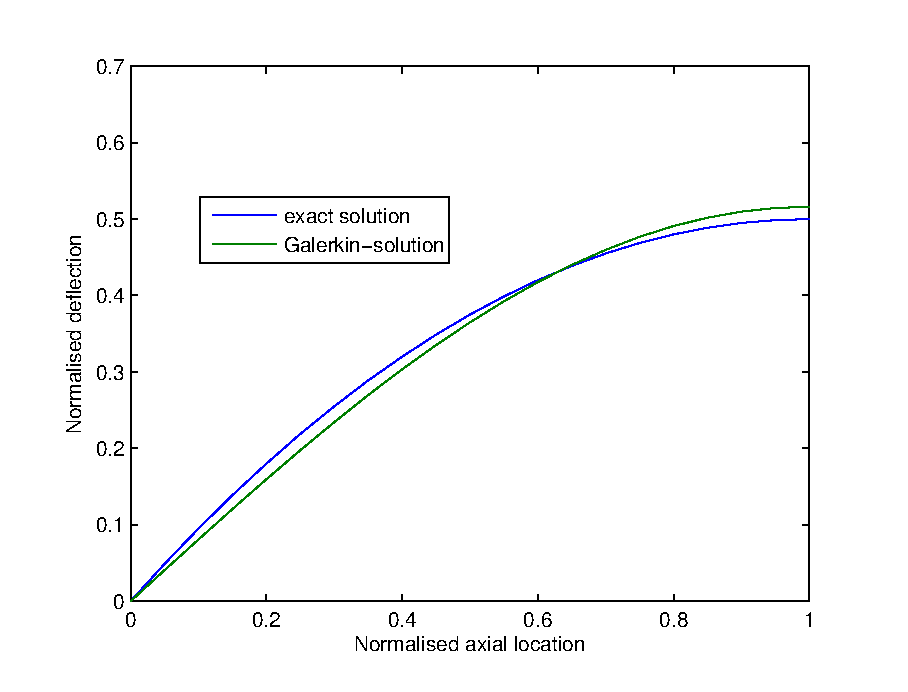
\includegraphics[scale=0.8]{ExactVSGalerkin.eps} 
\caption{The exact solution compared to the solution with a \eigenname{Galerkin}-weighted function}
\label{ExactVSGalerkin}
\end{center}
\end{figure}

{\bf Note:} The \eigenname{Galerkin}-solution here is made for a one-parameter trial function. For a more-parameter trial function with $û(x)\,=\,\sum c_i\,û_i(x)$ there would be weighted functions $W_i$ that make the approximative solution even more exact
\bigskip 

\subsection{Basic methods of my FEA-program}
In the following I will derive the equations used in my one-dimensional finite element program, first for the static case and then, much more complicated, for the dynamic case. I will only give a very short overview of the theoretical basics of FEA, the interested reader is referred to \cite{seshu} and \cite{ramamurty}.

\bigskip
\bigskip

\begin{minipage}{\textwidth}
    \begin{minipage}[t]{0.5\textwidth}
     
     Our one-dimensional beam element consists of two nodes at each end. Every node has two degrees of freedom as it can move normally to the beams axis and rotate around an axis normally to the grid. We define a vector $\vec{q}$  describing the deformations of one element and a vector $\vec{f}$ describing the forces and torques attached to the nodes:
    \end{minipage}
    \hfill
    %\mbox{\numexpr{0.95-#5}} geht vielleicht auch irgendwie
    \begin{minipage}[t]{0.5\textwidth}				%ehemals 0.45 [LARS]
      ~\\[-1ex]%fakezeile, um beide minipages mit der t-Zeile auszurichten
       
      \centerline{
      \psfrag {n1} {$n_1$}
      \psfrag{n2}{$n_2$}
      \psfrag{u1}{$u_1$}
      \psfrag{u2}{$u_2$}
      \psfrag{p1}{$\phi_1$}
      \psfrag{p2}{$\phi_2$}      
      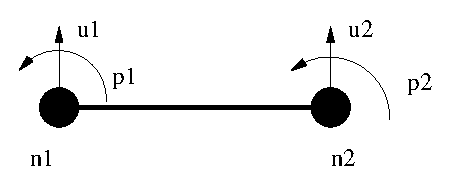
\includegraphics[scale=1]{beamElement1.eps}}
    \end{minipage}
  \end{minipage}

\begin{align}
\vec{q}&=\left(\begin{array}{c}
u_1 \\ 
\phi_1 \\ 
u_2 \\ 
\phi_2
\end{array} \right)&\vec{f}=\left(\begin{array}{c}
F_1 \\ 
M_1 \\ 
F_2 \\ 
M_2
\end{array}\right)\nonumber
\end{align}
where $u_1$ and $\phi_1$ are the displacements and rotations of the first node, respectively, and  $u_2$ and $\phi_2$ for the second node in the same manner. $F_i$ and $M_i$ are for the force and torques at node $i$.
\bigskip 

We now want to derive a matrix $\vec{k}$, so that $\vec{f}=\vec{k}*\vec{q}$. For that we will look at a beam, deformed in only one degree of freedom, based on the \begriff{Beam Theory} of \eigenname{Euler} and \eigenname{Bernoulli}. There are a whole bunch of books about the Beam Theory, the interested reader can read for example \cite{timoschenko}. For deriving the k-matrix we will deform our beam element four times, so it will just deform in one of the four degrees of freedom.\\
\bigskip
\begin{center}
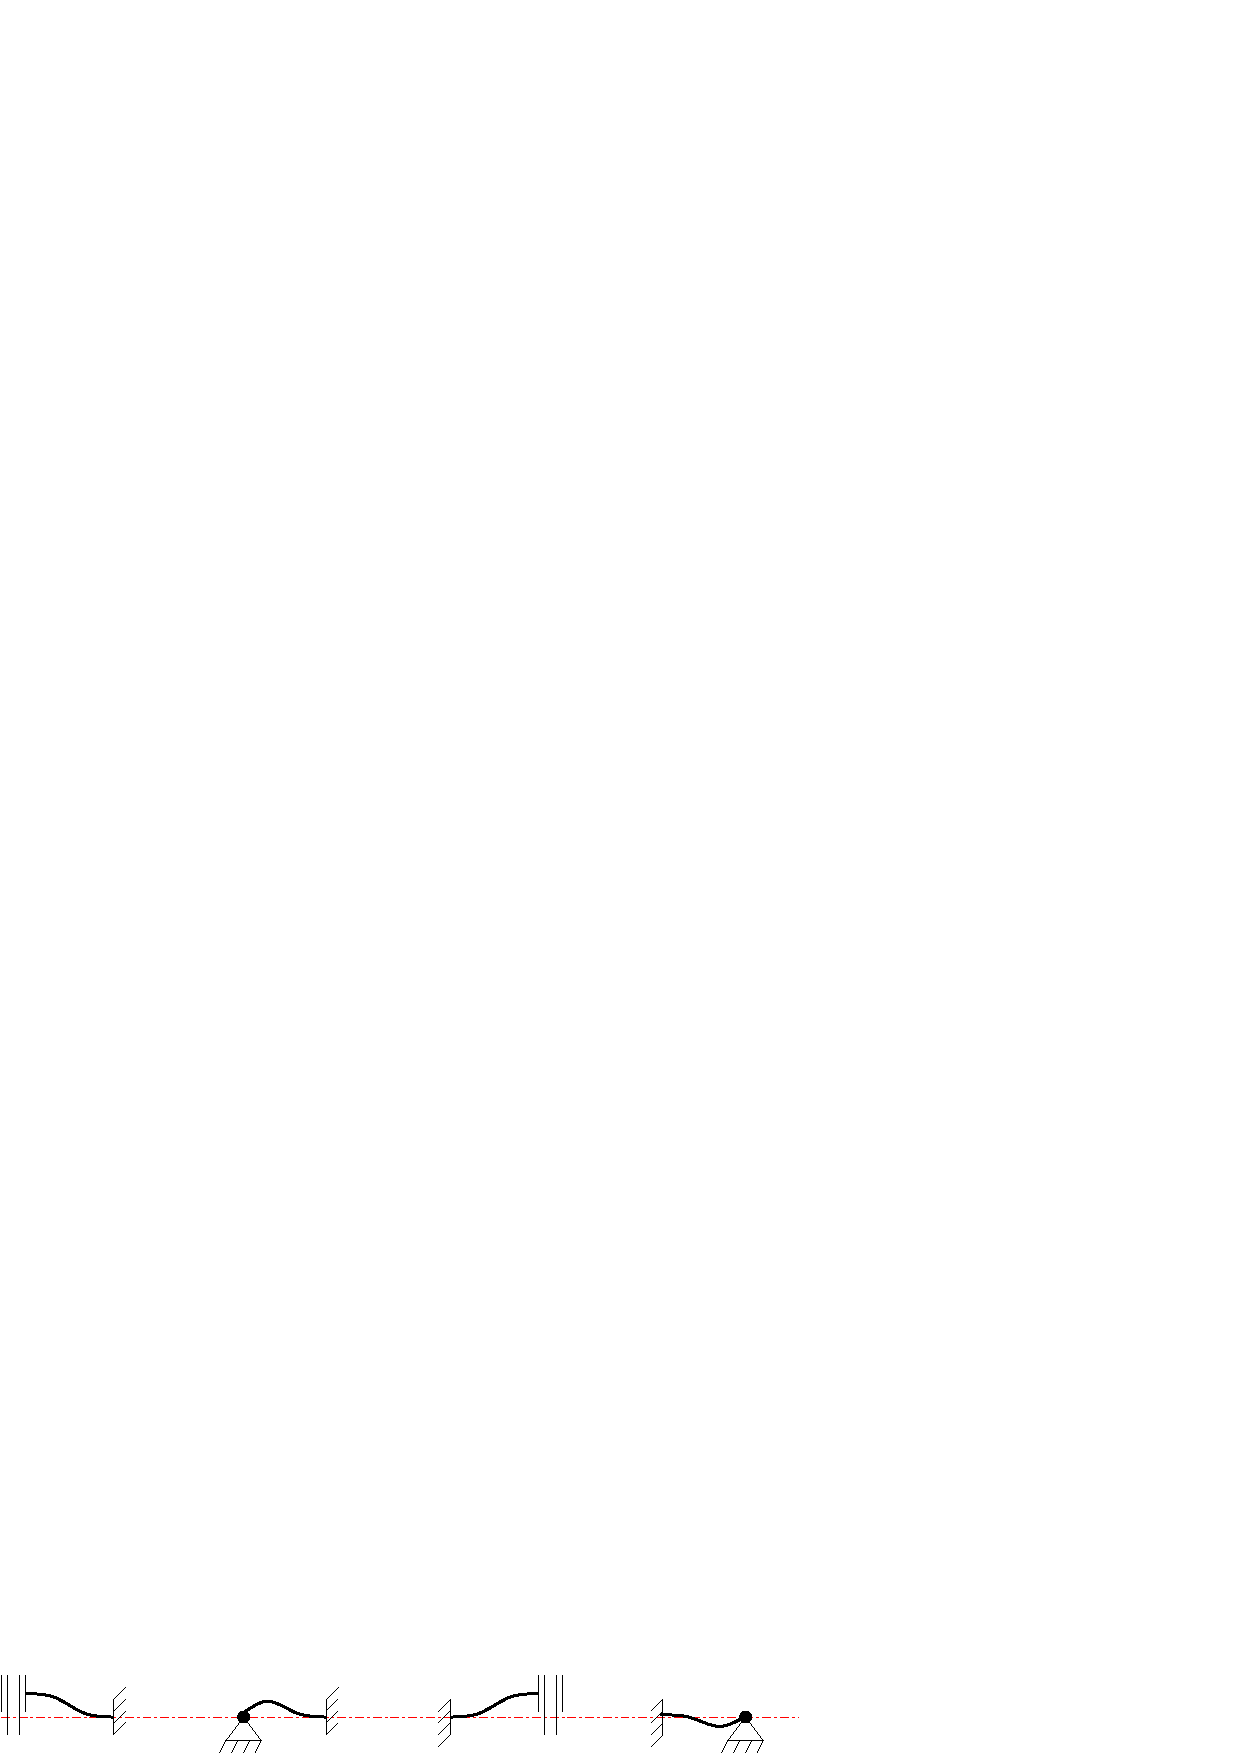
\includegraphics[scale=1.2]{fourDeformations}
\end{center}
\bigskip 

\begin{minipage}{\textwidth}
    \begin{minipage}[t]{0.5\textwidth}
     
     For a beam of lenght $l$ I will demonstrate the derivation of the k-matrix on an example of a beam which has only a displacement in its first degree of freedom.
    \end{minipage}
    \hfill
    %\mbox{\numexpr{0.95-#5}} geht vielleicht auch irgendwie
    \begin{minipage}[t]{0.5\textwidth}				%ehemals 0.45 [LARS]
      ~\\[-1ex]%fakezeile, um beide minipages mit der t-Zeile auszurichten
       
      \centerline{
      \psfrag{m1}{$M_1$}
      \psfrag{m2}{$M_2$}
      \psfrag{f1}{$F_1$}
      \psfrag{f2}{$F_2$}
      \psfrag{u1}{$u_1$}
      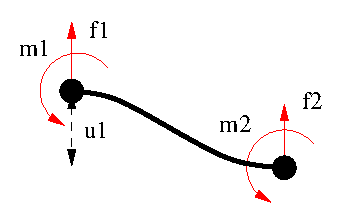
\includegraphics[scale=1]{deformBar1.eps}}
    \end{minipage}
  \end{minipage}
	\pagebreak
	
\begin{thebibliography}{9}

\bibitem {seshu}
P. Seshu,
\emph{Textbook of Finite Element Analysis}.
Prentice-Hall of India Private Limited, New Delhi,
Fourth Printing, 2006
\bibitem {ramamurty}
G. Ramamurty,
\emph{Applied Finite Element Analysis}.
I.K. International Publishing House Pvt. Ltd., New Delhi,
Second Edition, 2010
\bibitem {timoschenko}
S. Timoschenko,
\emph{History of strength of materials}.
McGraw-Hill, New-York,
1953

\end{thebibliography}

\end{document}